  \chapter{Revisão da Literatura}
  
  \section{NLP - Processamento de Linguagem Natural}
  O processamento de linguagem natural é uma vertente específica da Inteligência Artificial que utiliza conhecimentos da língua e de comunicação para melhorar a interação homem-máquina. É possível sintetizar o conceito de NLP como "a habilidade de um computador em processar a mesma linguagem que os humanos usam no cotidiano\cite{chatbot_definition}. Linguística, semântica, teoria da comunicação e processamento de sinais são algumas das áreas que auxiliam no processamento de linguagem natural.
  
  Um sistema conversacional é capaz de detectar \textit{intents} e \textit{entities}. O intent é o objetivo ou propósito da interação do usuário com o chatbot, enquanto uma entity é uma caraterística que adiciona valor a um intent\cite{jain2018convey} como demonstradona figura \ref{fig:nlp}.
  
  \begin{figure}[h!]
  	\begin{center}
  		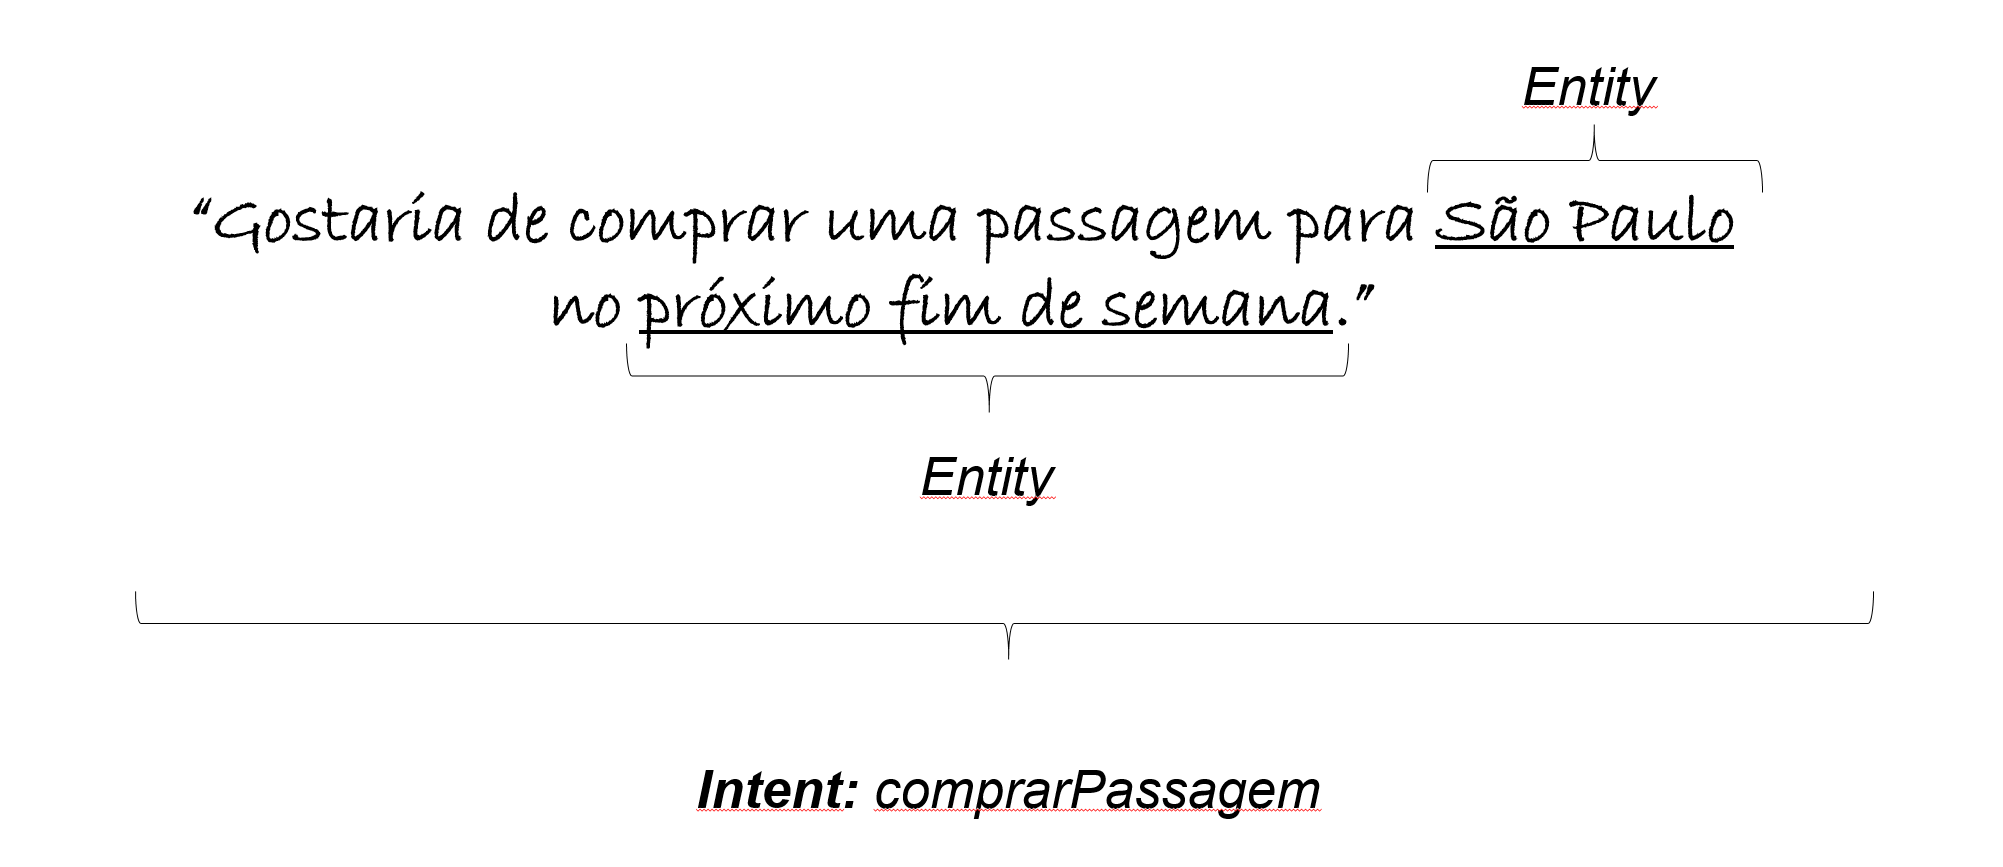
\includegraphics[width=0.95\linewidth]{images/nlp.png}
  		\caption{Interpretação de uma frase com processamento de linguagem natural}
  		\label{fig:nlp}
  	\end{center}
  \end{figure}
  
  A frase tem como objetivo (\textit{intent}) comprar uma passagem. Na frase, é possível identificar palavras que agregam para o objetivo de compra de passagem, como o destino (São Paulo) e data de partida (próximo fim de semana).
  
  \section{Chatbot baseado em regras}
  %Descrever todas as seções desse capítulo baseado nos artigos da base de artigos.
  %É um tipo de chatbot que funciona através de comandos específicos pré-definidos, tornando-os limitados às regras que ele conhece. De forma geral, os fluxos de conversa são bem definidos.
  \textit{Chatbots} baseados em regras são um tipo particular de \textit{bots} onde os fluxos de conversa são bem definidos e com opções mais limitadas de interação.
  
  A LEGO\footnote{https://www.messenger.com/t/LEGO}, fabricante de brinquedos infantis, possui um chatbot baseado em regras disponível na sua página do Messenger que é responsável por fornecer sugestões de presentes aos usuários baseado em um filtro de busca. O usuário fornece informações como localização, idade da criança e orçamento disponível e o \textit{bot} exibe as opções disponíveis.
  
  \section{Chatbots com inteligência artificial}
  Chatbots com inteligência artificial são aqueles que conseguem extrair informações de \textit{intents} e \textit{entities} de um texto enviado pelo usuário através de algoritmos de \textit{machine learning}, e também tomar decisões com base nos dados extraídos e o contexto da conversa.
  
  Em geral, os chatbots com inteligência artificial são treinados previamente para conhecer uma série de respostas para os \textit{intents} que ele irá atender. Sendo assim, ele não será capaz de responder a situações no qual ele não seja treinado.
  %Um chatbot inteligente é aquele que aprende com o tempo, ou com o treinamento. É caracterizado por tentar entender a linguagem natural de frases, em diversos contextos. Quanto mais treinado, melhor é o desempenho.
  
  \section{Uso do chatbot}
  %Escrever sobre o uso do chatbot em diferentes áreas.
  A aplicabilidade dos chatbots é, em geral, a mesma que qualquer outro sistema computacional, pois trata-se de uma interface de interação que permite execução de comandos de máquina e integração com outros tipos de sistema de software, como bancos de dados, por exemplo.
  
  O avanço no desenvolvimento das plataformas de bots, liderado principalmente pelo Facebook tornou possível a criação de chatbots que resolvem problemas reais da população, como é o caso do PrefeitoBot\cite{prefeitobot}. O PrefeitoBot é um bot para Messenger que traz informações sobre a prefeitura da cidade do Rio de Janeiro, como secretarias e horários de funcionamento. Além disso, também oferece um canal onde os usuários podem reportar ocorrências na cidade, como tombamento de árvores, alagamentos, poluição sonora, entre outras situações que o canal 1746 da cidade do Rio de Janeiro oferece atendimento.
  
  Chatbots também estão presentes no setor de varejo. As Casas Bahia lançou em 2017 o Bahianinho\footnote{https://www.facebook.com/CasasBahia/}, o chatbot da empresa responsável pelo atendimento dos consumidores através do \textit{Messenger}. Na época, sua principal função era enviar ofertas da Black Friday para os usuários, de acordo com suas preferências.
  
  No mesmo ano, o Rock in Rio criou o Roque\footnote{https://take.net/blog/take-notes/case-take-chatbot-no-rock-in-rio/}. O bot do festival interagiu com mais de 77 mil usuários, trocando cerca de 3 milhões de mensagens\footnote{https://take.net/blog/chatbots/cases-de-chatbots-famosos/} ao longo dos 7 dias de evento. Roque tirava dúvidas dos usuários, enviava notícias e prestava suporte aos participantes do festival e também aos que assistiam de casa.
  
  \section{Uso do chatbot na área médica}
  Os \textit{chatbots} podem desempenhar um papel estratégico na área médica. Em geral, por desempenhar um atendimento automatizado aos usuários que o utilizam, os \textit{chatbots} podem ser responsáveis por ser um canal disponível 24 horas por dia, podendo atender cada usuário de forma personalizada, oferecendo suporte a diversas situações da área da saúde como marcação de consultas, lembretes de medicação, dúvidas sobre doenças, etc.
  
  Hoje é possível encontrar diversos \textit{chatbots} aplicados a área médica como o \emph{HelpCare} \cite{helpcare}, que auxilia no tratamento de doenças crônicas como diabetes, colesterol alto e hipertensão arterial, e o \emph{MediBot} \cite{medibot}, que oferece informações sobre medicamentos.
  %xxxxxxxxxxxxxx
  